%\title{LaTeX Portrait Poster Template}
%%%%%%%%%%%%%%%%%%%%%%%%%%%%%%%%%%%%%%%%%
% a0poster Portrait Poster
% LaTeX Template
% Version 1.0 (22/06/13)
%
% The a0poster class was created by:
% Gerlinde Kettl and Matthias Weiser (tex@kettl.de)
% 
% This template has been downloaded from:
% http://www.LaTeXTemplates.com
%
% License:
% CC BY-NC-SA 3.0 (http://creativecommons.org/licenses/by-nc-sa/3.0/)
%
%%%%%%%%%%%%%%%%%%%%%%%%%%%%%%%%%%%%%%%%%

%----------------------------------------------------------------------------------------
%	PACKAGES AND OTHER DOCUMENT CONFIGURATIONS
%----------------------------------------------------------------------------------------

\documentclass[a0,portrait]{a0poster}

\usepackage{multicol} % This is so we can have multiple columns of text side-by-side
\columnsep=100pt % This is the amount of white space between the columns in the poster
\columnseprule=3pt % This is the thickness of the black line between the columns in the poster

\usepackage{caption}
\usepackage[svgnames]{xcolor} % Specify colors by their 'svgnames', for a full list of all colors available see here: http://www.latextemplates.com/svgnames-colors

\usepackage{times} % Use the times font
%\usepackage{palatino} % Uncomment to use the Palatino font

\usepackage{graphicx} % Required for including images
\graphicspath{{figures/}} % Location of the graphics files
\usepackage{booktabs} % Top and bottom rules for table
\usepackage[font=small,labelfont=bf]{caption} % Required for specifying captions to tables and figures
\usepackage{amsfonts, amsmath, amsthm, amssymb} % For math fonts, symbols and environments
\usepackage{wrapfig} % Allows wrapping text around tables and figures
\usepackage{algorithmic}
\usepackage[citestyle=numeric,bibstyle=numeric]{biblatex}
\addbibresource{sample.bib}



\begin{document}
	
	
	%----------------------------------------------------------------------------------------
	%	POSTER HEADER 
	%----------------------------------------------------------------------------------------
	
	% The header is divided into two boxes:
	% The first is 75% wide and houses the title, subtitle, names, university/organization and contact information
	% The second is 25% wide and houses a logo for your university/organization or a photo of you
	% The widths of these boxes can be easily edited to accommodate your content as you see fit
	
	\begin{minipage}[b]{0.75\linewidth}
		\veryHuge \color{NavyBlue} \textbf{Solovay-Kitaev's Algorithm} \color{Black}\\ % Title
		\Huge\textit{Operators Approximation}\\[2cm] % Subtitle
		\huge \textbf{David Cardozo, Juanita Duque \& Jonathan Ni\~no}\\[0.5cm] % Author(s)
		\huge Quantum Computing 2015-1. Professor: C\'esar Galindo\\[0.4cm] % University/organization
		
	\end{minipage}
	%
	\begin{minipage}[b]{0.25\linewidth}
		$$
\includegraphics[width=20cm]{figures/11215997_10153898950275550_1921299963_n.jpg}$$\\
	\end{minipage}
	
	\vspace{1cm} % A bit of extra whitespace between the header and poster content
	
	%----------------------------------------------------------------------------------------
	
	\begin{multicols}{2} % This is how many columns your poster will be broken into, a portrait poster is generally split into 2 columns
		
		%----------------------------------------------------------------------------------------
		%	ABSTRACT
		%----------------------------------------------------------------------------------------
		
		\color{Navy} % Navy color for the abstract
		
		\begin{abstract}
			In this work, we do a simple implementation of the Solovay-Kitaev's Algorithm using Python and Numpy for symbolic and numerical linear algebra evaluations, our discussion is mainly expository and it is mostly based on the C++ implementation in \cite{Harrow2001}, and the Python libraries in \cite{PaulPhamGit}.
		\end{abstract}
		
		%----------------------------------------------------------------------------------------
		%	INTRODUCTION
		%----------------------------------------------------------------------------------------
		
		\color{SaddleBrown} % SaddleBrown color for the introduction
		
		\section*{Introduction}
		
		\large{A} model of quantum computation is based on quantum circuits, composed by unitary operators.
		\\
		Any change over time can be expressed by an unitary matrix, without loss of generality we can normalize and suppose that this matrix has determinant equal to 1. The group of these matrices is named $SU(N)$, often called \emph{the special unitary group}. Although $ \operatorname{SU}(N)  $ has nice properties, we cannot simulate exactly all the matrices in that group because $SU(N)$ has the cardinality of the continuum \cite{Nielsen2000} and we can only simulate enumerable matrices in an exact manner.
		\\
		A very good workaround is to use the Solovay's Kitaev's algorithm, which consists in approximating any matrix in $SU(N)$ with a group of given matrices with a distance between the operators to be less than a given $\epsilon>0$. The algorithm works in polynomial time in classic computers and it is an important result for simulating a quantum computer or creating a quantum compiler.
		
		%----------------------------------------------------------------------------------------
		%	OBJECTIVES
		%----------------------------------------------------------------------------------------
		
		\color{DarkSlateGray} % DarkSlateGray color for the rest of the content
		
		\section*{Quantum Circuits}
		
		\large{A} quantum circuit over a basis $\mathcal{A}$ is a sequence $U_1[A_1],...,U_L[A_L]$ where $\mathcal{A}$ is a fixed set of unitary operators, $U_i\in \mathcal{A}$ and $A_i$ is and ordered set of qubits. It is the analogue of a circuit in classical computing and it is useful to represent quantum algorithms \cite{kitaev2002classical}.
		\\
		A quantum circuit is built upon quantum gates. Formally quantum gates are operators over one or two qbits, for example the Hadamard gates or the Pauli transformations. The gates that are normally chosen are those that can be potentially implemented as a physical phenomenom. Every circuit is build by various combinations of tensorial products and multiplication of quantum gates.
		\\
		$$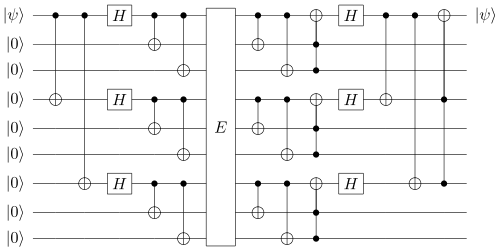
\includegraphics[width=30cm]{figures/500px-Shore_code_svg.png}$$
		\captionof{figure}{Example of a quantum circuit.}
		\label{circuit}
		
		\section*{Solovay-Kitaev's Theorem}
		
		\large{F}or any $A_1,...,A_l\in SU(N)$ such that $\left\langle A_1, . . . , A_{l}\right\rangle$ is dense in $SU(N)$, there exists a constant $C$ and a procedure for approximating any $U\in SU(N)$ to precision $\epsilon$ with a string of $A_1, . . . , A_l$ and their inverses of length no greater than $Clog^c(1/\epsilon)$, where $c\approx4$ and $C$ is independent of $U$ and $\epsilon$. This procedure can be implemented in polynomial time in $\log(1/\epsilon)$
		\\
		As a result we have that for any family of universal gates, there exists a constant $C$ such that any quantum circuit with $n$ arbitrary gates can be constructed from fewer than $ C_n \log^c(n) \log(1/\delta)$ universal gates if the probability of error is $\delta$.
		\\
		\color{SaddleBrown}
		
		
		%David's Apport
		
		
		One of the central results of quantum computation, the Solovay-Kitaev (SK) algorithm for the
		approximation of $SU(d)$ gates by a fixed, finite basis $\mathcal{B}$.
		Although many recent results have surpassed SK in terms of efficiency,
		many of them have, at their core, the base-level approximation of SK. Moreover, many techniques for analyzing
		and understanding quantum compilers were first developed for SK, which
		continues to be the best way to learn them. Finally, the overall
		structure of the original SK algorithm is so simple, it is surprising
		that it works so well.
		The essential structure of SK is to recursively generate nets of unitary
		operators with
		successively finer precision. At any given level of recursion, the input 
		gate is divided up into two halves which can be
		approximated with less precision, but whose errors cancel out
		when the approximated halves are recombined. Our pseudo-code 
		in Figure \ref{sk-code} and explanation
		follows the exposition in \cite{Dawson2005} and \cite{Harrow2001}.
		
		\color{DarkSlateGray} 
		
		Since the recursion must eventually bottom out, we must precompute some sequences
		of gates from $\mathcal{B}$ up to length $l_0$. This is the classical
		preprocessing step which requires upfront storage space for this
		coarsest-grained net, where
		each sequence is no more than $\epsilon_0$ from its nearest neighbor. According
		to \cite{Dawson2005} the values of $l_0=16$ and $\epsilon_0 = 0.14$ using
		operator norm distance is sufficient for most applications.
		This step can be
		done offline and reused across multiple runs of the compiler, assuming
		$\mathcal{B}$ for your quantum computer doesn't change.
		
		The BASIC-APPROX function below does a lookup (e.g. using some kd-tree search
		maneuvers through higher-dimensional vector spaces) using this $\epsilon_0$-net,
		and all higher recursive calls to SK are effectively constructing
		finer $\epsilon$-nets ``on the fly'' as needed.
		
		The FACTOR function performs a balanced group commutator decomposition,
		$U = ABA^\dagger B^\dagger$, and then recursively approximates the $A$ and $B$
		operators, again using SK. We denote by $\tilde{U}_i$ the approximation
		of $U$ using $i$ levels of SK recursion. When they are multiplied
		together again, along with their inverses, their errors (which go like
		$\epsilon$) are symmetric and cancel out in such a way that the resulting
		product $U$ has errors which go like $\epsilon^2$, using the properties of
		the balanced group commutator. In this manner, we can
		eventually sharpen our desired error down to any value. A
		geometric decomposition is used in the Dawson-Nielsen implementation \cite{Dawson2005},
		while one based on a Baker-Campbell-Hausdorff approximation is used in the
		Harrow implementation \cite{Harrow2001} following
		Nielsen and Chuang \cite{Nielsen2000}. It is not
		known which method converges more quickly to a desired gate in general.
		
		
		%endof
		
		\color{SaddleBrown}
		
		\section*{Pseudocode}
		The pseudocode in which the implementation was based is the following
		
		\begin{minipage}{50cm}
			\begin{algorithmic}[1]
				\STATE \textsc{function} $\tilde{U}_i \leftarrow$ SK$(U,i)$
				\IF{$i = 0$}
				\STATE $\tilde{U}_i \leftarrow $ BASIC-APPROX$(U)$
				\ELSE
				\STATE $\tilde{U}_{i-1} \leftarrow$ SK$(U, i-1)$
				\STATE $A,B \leftarrow $ FACTOR$(U\tilde{U}^\dagger_{i-1})$
				\STATE $\tilde{A}_{i-1} \leftarrow $ SK$(A, i-1)$
				\STATE $\tilde{B}_{i-1} \leftarrow $ SK$(B, i-1)$
				\STATE $\tilde{U}_i \leftarrow \tilde{A}_{i-1}\tilde{B}_{i-1}\tilde{A}^\dagger_{i-1}\tilde{B}^\dagger_{i-1}\tilde{U}_{i-1}$
				\ENDIF
				\STATE return $\tilde{U}_i$
			\end{algorithmic}
			\centering
			\captionof{figure}{Pseudo-code for the Solovay-Kitaev algorithm \cite{Dawson2005}.}
			\label{sk-code}
		\end{minipage}
		
		
		
		\color{SaddleBrown} % SaddleBrown color for the conclusions to make them stand out
		
		
		\color{DarkSlateGray} % Set the color back to DarkSlateGray for the rest of the content
		
		\section*{Implementation}
		
		As mentioned above the implementation of the algorithm was develop in Python using a previous work by Paul Pham. The program shows the exact sequences of matrices used to approximate the unitary operator and gives the distance between the approximation and the original matrix. An improvement made was the use of a $k$-$d$-tree to optimize the search time of the original algorithm. The algorithm is performed within polynomial time.   
		
		
		\color{SaddleBrown}
		
		
		\section*{Observations and Conclusions}
		
		We often have a very small trace distance in our calculations of the approximation (of the order $ \approx 0.23 $), which as expected, is very good for applications and future work. On the other hand, the use of Python for this implementations decreases the speed considerably compared with the C++ implementation. We don't see this implementation feasible for working with $ SU(4) $ or $ SU(8) $, mainly because generating the sequences associated to these groups, generates an 'out of memory' situation and the process takes an extremely long time.  
		%\section*{References}
		
		\color{DarkSlateGray}
		
		\printbibliography
		
		
		
		%----------------------------------------------------------------------------------------
		
	\end{multicols}
\end{document}